This use-case is the implementation of the scenario of \emph{voluntary-automatic}
presented in the matrix  in \autoref{tab:matrix}.

For the Automatic use case we choose to implement a widely used feature detection
algorithm, the \ac{SIFT}. To perform this load intensive algorithm we used the
power of the \ac{WebCL} framework to greatly speedup the computation.

% Come funziona
%% Creazione della libreria per comunicare con WebCl
%% Librearia per le operazioni sulle immagini usango WebCL
%% implementazione nella libreria dell'algoritmo
%% Fasi dell'algoritmo


\begin{figure}[htb]
    \centering
    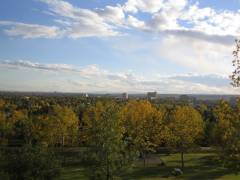
\includegraphics[width=\columnwidth]{Automatic1}
    \caption{The interface of the automatic use-case.}
    \label{fig:Automatic1}
\end{figure}


\begin{figure}[htb]
    \centering
    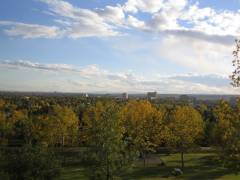
\includegraphics[width=\columnwidth]{Automatic3}
    \caption{Step results of the algorithm.}
    \label{fig:Automatic1}
\end{figure}


\begin{figure}[htb]
    \centering
    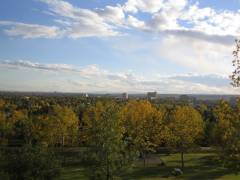
\includegraphics[width=\columnwidth]{Automatic3}
    \caption{Comparison with the reference data.}
    \label{fig:Automatic1}
\end{figure}


% 

%Our scenario is to detect features over 100.000 images using this algorithm


\subsubsection{Benchmark}
%non è possibile una vera comparazione data la velocità